\documentclass[11pt,a4paper]{article}

\usepackage[T1]{fontenc}
\usepackage{lmodern}
\usepackage{amsmath,amssymb,amsthm}
\usepackage{geometry}
\usepackage{xcolor}
\usepackage{tikz}
\usetikzlibrary{calc}
\usepackage{float}
\usepackage[colorlinks=true,linkcolor=blue,urlcolor=blue,citecolor=blue]{hyperref}

\geometry{margin=2.4cm}

\definecolor{lampA}{RGB}{198,43,42}
\definecolor{lampB}{RGB}{44,93,197}

\newtheorem{theorem}{Theorem}[section]
\newtheorem{lemma}[theorem]{Lemma}
\newtheorem{proposition}[theorem]{Proposition}
\theoremstyle{definition}
\newtheorem{definition}[theorem]{Definition}

\title{One More Step on W\"astlund's Geometric Proof of the Basel Problem}
\author{YeXiaoRain\thanks{Independent researcher, Chengdu, Sichuan, China.
  \texttt{yexiaorain@gmail.com}}}
\date{November 20, 2026}

\begin{document}

\maketitle

\begin{abstract}
W\"astlund's geometric proof of the Basel problem doubles a circle again and again and
replaces each lamp by two equivalent ones, so that the brightness at the observation point
never changes; in the limit the figure yields the sum of the reciprocal squares of the
\emph{odd} integers, and one further algebraic step is needed to reach the full series.
We modify the doubling by adding a single lamp at the point of the new circle antipodal to
the observer. That position is precisely the one the replacement cannot produce, so exactly
one lamp is missing each round; the added lamps stand at distances that double every time,
so their contributions form a geometric series, while the limiting line carries a lamp at
every nonzero integer point. Equating the two brightnesses gives $\sum_{n\ge1}1/n^{2}=\pi^{2}/6$
directly off the figure, with no detour through the odd terms.
\end{abstract}

\begin{center}
\small
\textbf{MSC 2020:} 51M04 (primary); 40A05, 11A25, 01A50\\[0.3em]
\textbf{Keywords:} Basel problem; geometric proof; inverse-square law;
W\"astlund's construction; infinite series
\end{center}

\section{Introduction}

The Basel problem asks for the sum of the reciprocal squares of the positive integers:
\begin{equation}
  S=\sum_{n=1}^{\infty}\frac{1}{n^{2}}
   =1+\frac{1}{2^{2}}+\frac{1}{3^{2}}+\frac{1}{4^{2}}+\cdots .
  \label{eq:basel}
\end{equation}
Mengoli posed it in 1644 and Euler evaluated the sum in 1735 as $\pi^{2}/6$. The left-hand
side is built out of integers alone, while the right-hand side is a circle constant, so one
expects a geometric reading of the identity.

Such a reading was given by W\"astlund \cite{wastlund} in a short note and popularised by
3Blue1Brown \cite{threeblueonebrown}. It uses nothing beyond Euclidean geometry: circles,
chords, right angles, and the inverse-square law for light. A lamp on a circle is a point
source, the common tangent point $P$ of two circles is the observer, and a term $1/d^{2}$ is
read as the brightness that a lamp at distance $d$ delivers at $P$. Doubling the circle
replaces every lamp by two equivalent ones on the larger circle, so the total brightness at
$P$ is preserved; in the limit the circle flattens into a line and its lamps fall on the odd
integers.

Normalise the construction so that the circle of circumference $2$ carries a single lamp, at
the point antipodal to $P$, at distance $2/\pi$. What the figure then delivers is the odd
terms.

\begin{theorem}[W\"astlund]\label{thm:wastlund}
With the normalisation above, the construction gives
\begin{equation}
  \sum_{k=0}^{\infty}\frac{1}{(2k+1)^{2}}=\frac{\pi^{2}}{8}.
  \label{eq:odd-sum}
\end{equation}
\end{theorem}

Getting $S$ out of Theorem \ref{thm:wastlund} costs one algebraic remark: the even terms are
$\frac14 S$, so $\frac34 S=\frac{\pi^{2}}{8}$. That remark is the only non-geometric step in
the whole argument, and it is the step this note removes.

\begin{theorem}[this note]\label{thm:direct}
Modify the doubling as follows: at every round, after the lamps have been replaced by their
images on the larger circle, add one lamp at the point of that circle antipodal to $P$. Then
every nonzero integer point of the limiting line carries a lamp, the brightness they deliver
at $P$ equals the brightness of the added lamps, and
\begin{equation}
  S=\frac{1}{2}\left(\frac{\pi^{2}}{2^{2}}+\frac{\pi^{2}}{4^{2}}+\frac{\pi^{2}}{8^{2}}+\cdots\right)
   =\frac{\pi^{2}}{6}.
  \label{eq:direct}
\end{equation}
The factor $\frac12$ is there because the line carries each distance twice, at $n$ and at $-n$:
what the picture delivers is $2S$. The term of round $k$ is the brightness $\pi^{2}/(2^{k+1})^{2}$
of the single lamp added in that round, which stands at distance $2^{k+1}/\pi$ from $P$.
\end{theorem}

Only one lamp has to be added each round, and it always sits in the same place: the antipodal
position is exactly the one the replacement cannot produce, since its preimage would be a lamp
at $P$ itself. Every other integer position is filled exactly once.

Equalities \eqref{eq:basel} and $\pi^{2}/6$ have been reached by many different routes;
Kalman's survey collects six of them \cite{kalman} and Matsuoka gives an elementary one
\cite{matsuoka}. Closest in spirit to the picture below is Dumont's heuristic argument,
made rigorous by Komornik, which ties the Gregory--Leibniz and Basel sums together
\cite{komornik}.

Every account of this geometric route that we were able to find has the same shape. W\"astlund's
own note \cite{wastlund}, the geometric-proof section of the Wikipedia article \cite{wikipedia},
and the video version by 3Blue1Brown \cite{threeblueonebrown} all carry the doubling to the
limit, read off the brightness of the lamps at the odd integers, and then recover $S$ from the
observation that the even terms are a quarter of it. As far as the author could find, no earlier
figure of this kind gives the whole series itself: each of these accounts stops at a sub-series
and closes with the same two lines of algebra, which is what \eqref{eq:direct} avoids. None of
them is the route we modify: what follows concerns only W\"astlund's construction
\cite{wastlund}.

Section \ref{sec:wastlund} reproduces W\"astlund's proof; Section \ref{sec:one-more-step}
contains the modification and the proof of Theorem \ref{thm:direct}, which is the only new
content of this note.

\section{W\"astlund's construction}\label{sec:wastlund}

\subsection{Brightness and the inverse-square law}

A lamp is a point source emitting a total flux $L$ equally in all directions, and the
observer receives it on a small screen perpendicular to the incoming rays. At distance $r$
the flux is spread over a sphere of area $4\pi r^{2}$, so the brightness per unit area is
\begin{equation}
  B(r)=\frac{L}{4\pi r^{2}}\propto\frac{1}{r^{2}}.
  \label{eq:inverse-square}
\end{equation}
Doubling the distance leaves a quarter of the brightness. Throughout, the distance of a lamp
is measured from the observation point $P$, and a sum of terms $1/d^{2}$ is read as the total
brightness at $P$.

\begin{definition}[lamps, brightness, equivalence]\label{def:lamps}
Fix a point $P$ in the plane, called the \emph{observation point}. A \emph{lamp} is a point
source placed at some $Q\neq P$, and its \emph{brightness at $P$} is the quantity
$1/PQ^{2}$. The \emph{total brightness} of a finite or countable set of lamps is the sum of
their brightnesses. Two lamps $S_{1},S_{2}$ are \emph{equivalent} to a lamp $R$ (at $P$) if
$1/PS_{1}^{2}+1/PS_{2}^{2}=1/PR^{2}$. If a circle through $P$ has centre $O$, the point of the
circle diametrically opposite $P$ is called the \emph{antipodal position} of $P$.
\end{definition}

With this vocabulary, replacing a lamp by two equivalent ones leaves the total brightness
unchanged, and all that must be checked in a replacement step is the inverse Pythagorean
identity of Lemma~\ref{lem:inverse-pythagoras}.

\subsection{The inverse Pythagorean theorem}

\begin{lemma}[inverse Pythagorean]\label{lem:inverse-pythagoras}
Let $a$ and $b$ be the legs of a right triangle, $c$ its hypotenuse, and $h$ the altitude to
the hypotenuse. Then
\begin{equation}
  \frac{1}{h^{2}}
  =\frac{c^{2}}{a^{2}b^{2}}
  =\frac{a^{2}+b^{2}}{a^{2}b^{2}}
  =\frac{1}{a^{2}}+\frac{1}{b^{2}}.
  \label{eq:inverse-pythagoras}
\end{equation}
\end{lemma}

\begin{proof}
Equating the two expressions for the area gives $ab=ch$, hence $c^{2}h^{2}=a^{2}b^{2}$;
substituting $c^{2}=a^{2}+b^{2}$ yields \eqref{eq:inverse-pythagoras}.
\end{proof}

\begin{figure}[htbp]
\centering
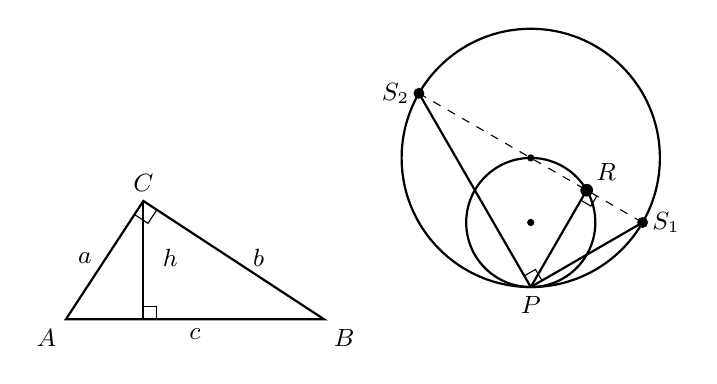
\begin{tikzpicture}[scale=0.82, every node/.style={font=\small}]
  \begin{scope}
    \coordinate (A) at (0,0);
    \coordinate (B) at (4,0);
    \coordinate (C) at (1.2,1.833);
    \coordinate (H) at (1.2,0);
    \draw[thick] (A)--(B)--(C)--cycle;
    \draw[thick] (C)--(H);
    \draw (1.4,0)--(1.4,0.2)--(1.2,0.2);
    \draw (1.063,1.624)--(1.272,1.487)--(1.409,1.696);
    \node[left] at (0.55,0.95) {$a$};
    \node[right] at (2.75,0.95) {$b$};
    \node[right] at (1.35,0.95) {$h$};
    \node[below] at (2,0) {$c$};
    \node[below left] at (A) {$A$};
    \node[below right] at (B) {$B$};
    \node[above] at (C) {$C$};
  \end{scope}

  \begin{scope}[shift={(7.2,0.5)}]
    \coordinate (P) at (0,0);
    \coordinate (O1) at (0,1);
    \coordinate (O2) at (0,2);
    \draw[thick] (O1) circle (1);
    \draw[thick] (O2) circle (2);
    \coordinate (R) at (0.866,1.5);
    \coordinate (S1) at (1.732,1);
    \coordinate (S2) at (-1.732,3);
    \draw[dashed] (S2)--(S1);
    \draw[thick] (P)--(R);
    \draw[thick] (P)--(S1);
    \draw[thick] (P)--(S2);
    \fill (R) circle (2.8pt);
    \fill (S1) circle (2.4pt);
    \fill (S2) circle (2.4pt);
    \fill (O1) circle (1.6pt);
    \fill (O2) circle (1.6pt);
    \draw (0.776,1.344)--(0.932,1.254)--(1.022,1.410);
    \draw (0.173,0.1)--(0.073,0.273)--(-0.1,0.173);
    \node[above right] at (R) {$R$};
    \node[right] at (S1) {$S_1$};
    \node[left] at (S2) {$S_2$};
    \node[below] at (P) {$P$};
  \end{scope}
\end{tikzpicture}
\caption{Left: the inverse Pythagorean theorem. Right: the replacement of
Lemma \ref{lem:replacement}.}
\label{fig:circle-replacement}
\end{figure}

\subsection{One lamp replaced by two equivalent lamps}

\begin{lemma}[replacement]\label{lem:replacement}
Let $C_{1}$ and $C_{2}$ be circles of radii $r_{1}$ and $r_{2}=2r_{1}$, tangent at the
observer $P$, and let $R$ be a lamp on $C_{1}$. The line through $R$ perpendicular to $PR$
meets $C_{2}$ in two points $S_{1}$ and $S_{2}$, and
\begin{equation}
  \underbrace{\frac{1}{PR^{2}}}_{\text{one lamp on }C_{1}}
  \;=\;
  \underbrace{\frac{1}{PS_{1}^{2}}+\frac{1}{PS_{2}^{2}}}_{\text{two lamps on }C_{2}}.
  \label{eq:replacement}
\end{equation}
\end{lemma}

\begin{proof}
The point of $C_{1}$ antipodal to $P$ lies on the line of centres at distance
$2r_{1}=r_{2}$ from $P$, so it is the centre $O_{2}$ of $C_{2}$. Because $PO_{2}$ is a
diameter of $C_{1}$, the angle $PRO_{2}$ is a right angle: the perpendicular to $PR$ at $R$
is the line $RO_{2}$, and it cuts $C_{2}$ in the two endpoints of a diameter. Thus $S_{1}S_{2}$
is a diameter of $C_{2}$, and since $P$ lies on $C_{2}$ the angle $S_{1}PS_{2}$ is a right
angle with $PR$ as the altitude to its hypotenuse. Lemma
\ref{lem:inverse-pythagoras} applied to the triangle $PS_{1}S_{2}$ is exactly
\eqref{eq:replacement}.
\end{proof}

In other words, one lamp on the small circle may be replaced by two lamps on the large one
without changing the brightness at $P$.

\subsection{Doubling: $N$ division points become $2N$}

\begin{lemma}[doubling]\label{lem:doubling}
Place lamps at $N$ equally spaced points of $C_{1}$ and replace each of them by its two
images on $C_{2}$ as in Lemma \ref{lem:replacement}. Those images are the $2N$ equally spaced
points of $C_{2}$ that correspond to them, and the total brightness at $P$ is unchanged.
\end{lemma}

\begin{proof}
The image pair of a lamp $R$ is the diameter of $C_{2}$ through $R$ and $O_{2}$, so the whole
configuration is a set of rays through $O_{2}$. Since $O_{2}$ lies on $C_{1}$, the angles
between consecutive rays are inscribed angles of $C_{1}$ standing on equal chords, hence
equal; the very same angles are central angles of $C_{2}$, so the $2N$ points in which the
rays meet $C_{2}$ cut $C_{2}$ into equal arcs. Brightness is preserved lamp by lamp by
Lemma \ref{lem:replacement}.
\end{proof}

The word \emph{corresponding} matters. The $2N$ points are produced from the $N$ lamps one at
a time; choosing an arbitrary set of $2N$ division points would not preserve the brightness.

\begin{figure}[htbp]
\centering
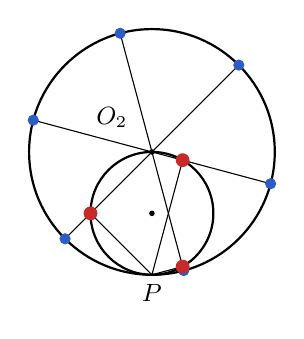
\begin{tikzpicture}[scale=0.78, every node/.style={font=\small}]
  \coordinate (P) at (0,0);
  \coordinate (O1) at (0,1);
  \coordinate (O2) at (0,2);
  \draw[thick] (O1) circle (1);
  \draw[thick] (O2) circle (2);
  \coordinate (R1) at (0.5,1.866);
  \coordinate (R2) at (0.5,0.134);
  \coordinate (R3) at (-1,1);
  \foreach \a [evaluate=\a as \c using {\a+180}] in {45,105,165}
    \draw[thin] ($(O2)+(\a:2)$)--($(O2)+(\c:2)$);
  \draw[thin] (P)--(R1);
  \draw[thin] (P)--(R2);
  \draw[thin] (P)--(R3);
  \foreach \a in {45,105,165,225,285,345}
    \fill[lampB] ($(O2)+(\a:2)$) circle (2.6pt);
  \fill[lampA] (R1) circle (3.2pt);
  \fill[lampA] (R2) circle (3.2pt);
  \fill[lampA] (R3) circle (3.2pt);
  \fill (O1) circle (1.3pt);
  \fill (O2) circle (1.3pt);
  \node[above left] at ($(O2)+(-0.24,0.24)$) {$O_2$};
  \node[below] at (P) {$P$};
\end{tikzpicture}
\caption{The $3$ division points of the small circle against the corresponding $6$ points of
the large one.}
\label{fig:doubling}
\end{figure}

\subsection{The limit: the circle becomes a line}

Take the circle of circumference $2$, that is, of radius $R_{0}=1/\pi$, with its single lamp
at the point antipodal to $P$. That lamp is at distance $2/\pi$, so the total brightness at
$P$ is
\begin{equation}
  \frac{1}{d^{2}}=\frac{1}{(2/\pi)^{2}}=\frac{\pi^{2}}{4}.
  \label{eq:first-lamp}
\end{equation}

\begin{figure}[H]
\centering
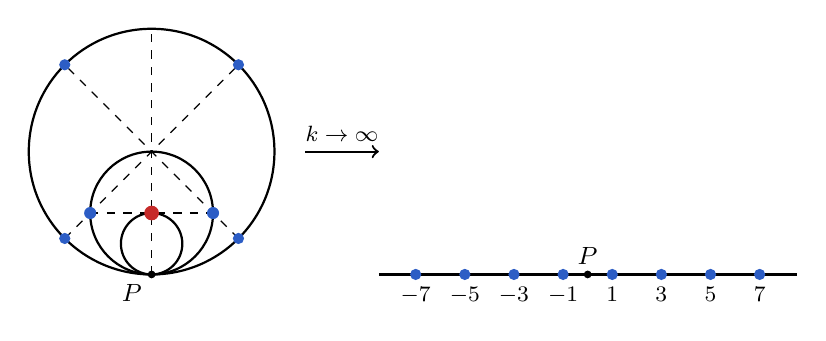
\begin{tikzpicture}[scale=0.78, every node/.style={font=\small}]
  \draw[dashed] (0,0)--(0,4);
  \draw[thick] (0,0.5) circle (0.5);
  \draw[thick] (0,1) circle (1);
  \draw[thick] (0,2) circle (2);
  \draw[thin,dashed] (-1,1)--(1,1);
  \draw[thin,dashed] (1.414,0.586)--(-1.414,3.414);
  \draw[thin,dashed] (-1.414,0.586)--(1.414,3.414);
  \fill[lampB] (1.414,0.586) circle (2.6pt);
  \fill[lampB] (-1.414,0.586) circle (2.6pt);
  \fill[lampB] (1.414,3.414) circle (2.6pt);
  \fill[lampB] (-1.414,3.414) circle (2.6pt);
  \fill[lampB] (1,1) circle (2.8pt);
  \fill[lampB] (-1,1) circle (2.8pt);
  \fill[lampA] (0,1) circle (3.4pt);
  \fill (0,0) circle (1.8pt);
  \node[below left] at (0,0) {$P$};
  \draw[->,thick] (2.5,2)--(3.7,2);
  \node[above,font=\footnotesize] at (3.1,2) {$k\to\infty$};
  \begin{scope}[shift={(7.1,0)}]
    \draw[thick] (-3.4,0)--(3.4,0);
    \fill (0,0) circle (1.8pt);
    \node[above] at (0,0) {$P$};
    \foreach \x/\lab in {-2.8/-7,-2.0/-5,-1.2/-3,-0.4/-1,0.4/1,1.2/3,2.0/5,2.8/7} {
      \fill[lampB] (\x,0) circle (2.6pt);
      \node[below,font=\footnotesize] at (\x,-0.05) {$\lab$};
    }
  \end{scope}
\end{tikzpicture}
\caption{Doubling the radius until the circle flattens into the tangent line.}
\label{fig:doubling-limit}
\end{figure}

Each doubling preserves this total, and after $k$ doublings the lamps of the circle of
circumference $2^{k+1}$ stand at arc-length distances $1,3,5,\dots$ from $P$. As $k\to\infty$
the circle approaches its tangent line at $P$, chord lengths tend to arc lengths, and the
lamps fall at $\pm1,\pm3,\pm5,\dots$ on that line (Figure \ref{fig:doubling-limit}). Hence
\begin{equation}
  2\left(1+\frac{1}{3^{2}}+\frac{1}{5^{2}}+\cdots\right)=\frac{\pi^{2}}{4},
  \label{eq:odd-limit}
\end{equation}
and dividing by $2$ proves Theorem \ref{thm:wastlund}.

\subsection{Back to the Basel problem}

The even terms of \eqref{eq:basel} are $\frac14$ of the whole series, so with
\eqref{eq:odd-sum}
\begin{equation}
  \resizebox{\textwidth}{!}{$
  \begin{array}{r*{21}{c}r}
    &1&&&+&\frac{1}{3^{2}}&&&+&\frac{1}{5^{2}}&&&+&\frac{1}{7^{2}}&&&+&\frac{1}{9^{2}}
    &&&+&\cdots&=\frac{\pi^{2}}{8}\\[14pt]
    S=&1&+&\frac{1}{2^{2}}&+&\frac{1}{3^{2}}&+&\frac{1}{4^{2}}&+&\frac{1}{5^{2}}
    &+&\frac{1}{6^{2}}&+&\frac{1}{7^{2}}&+&\frac{1}{8^{2}}&+&\frac{1}{9^{2}}
    &+&\frac{1}{10^{2}}&+&\cdots&\\[20pt]
    \frac{1}{4}S=&&&\frac{1}{2^{2}}&&&+&\frac{1}{4^{2}}&&&+&\frac{1}{6^{2}}
    &&&+&\frac{1}{8^{2}}&&&+&\frac{1}{10^{2}}&+&\cdots&
  \end{array}$}
  \label{eq:odd-even}
\end{equation}
and therefore $S=\frac{\pi^{2}}{8}\cdot\frac{1}{1-\frac14}=\frac{\pi^{2}}{6}$. This last
computation is the algebraic step that Theorem \ref{thm:direct} below avoids:
\eqref{eq:odd-even} trades $S$ for $\frac34 S$, and with it the information carried by the
figure becomes a subseries.

\section{One more step: a single added lamp each round}\label{sec:one-more-step}

Section \ref{sec:wastlund} hands over the odd terms only. We change the doubling rule at one
point: after the lamps of a circle have been replaced by their images on the doubled circle,
add one lamp at the point of the doubled circle antipodal to $P$.

\begin{lemma}[the missing position]\label{lem:missing}
Let the $k$-th circle have circumference $C=2^{k+1}$, radius $2^{k}/\pi$, and lamps at the
arc positions $s=1,2,\dots,C-1$ measured from $P$. Under the replacement of Lemma
\ref{lem:doubling} the lamps of the doubled circle occupy every integer arc position
$1,\dots,2C-1$ except $s=C$, which is the point antipodal to $P$; and no lamp of the
$k$-th circle can be mapped there.
\end{lemma}

\begin{proof}
A lamp at arc position $s$ on the $k$-th circle is replaced by the two endpoints of the
diameter of the doubled circle through it, which stand at arc positions $s$ and $s+C$; this
covers each of $1,\dots,2C-1$ with $s\ne C$ exactly once. The point at arc position $C$ is the
far end of the diameter through $P$, that is, the line of centres; the other point of that
line on the $k$-th circle is $P$ itself, which carries no lamp. So the antipodal position has
no preimage.
\end{proof}

\begin{proposition}[brightness of the added lamps]\label{prop:added}
The lamp added at round $k$ stands at distance $2^{k+1}/\pi$ from $P$, hence contributes
$\pi^{2}/(2^{k+1})^{2}$ by \eqref{eq:inverse-square}, and the added lamps together give
\begin{equation}
  B=\frac{\pi^{2}}{2^{2}}+\frac{\pi^{2}}{4^{2}}+\frac{\pi^{2}}{8^{2}}+\cdots
   =\frac{\pi^{2}}{4}\cdot\frac{1}{1-\frac14}
   =\frac{\pi^{2}}{3}.
  \label{eq:supplement-brightness}
\end{equation}
Each term is the brightness at $P$ of one of the red lamps in Figure \ref{fig:onepic}, one term
per round, in the order in which the circles are drawn.
\end{proposition}

\begin{proof}
The distance from $P$ to the antipode is the diameter of the $k$-th circle, which is
$2^{k+1}/\pi$. The remaining sum is geometric with ratio $\frac14$.
\end{proof}

\begin{proof}[Proof of Theorem \ref{thm:direct}]
As the radius tends to infinity the circles flatten into the tangent line at $P$, chords tend
to arcs, and by Lemma \ref{lem:missing} every integer position is lit: the limiting line
carries lamps at all nonzero integers, at distances $1,2,3,\dots$ from $P$
(Figure \ref{fig:onepic}). The brightness they deliver at $P$ is
$\sum_{n\neq0}1/n^{2}=2S$. By Lemma \ref{lem:replacement} the replacement never changes the
brightness at $P$, so this total equals the brightness \eqref{eq:supplement-brightness} of the
lamps that had to be added. Hence
\begin{equation*}
  S=\frac{B}{2}
   =\frac{1}{2}\left(\frac{\pi^{2}}{2^{2}}+\frac{\pi^{2}}{4^{2}}+\frac{\pi^{2}}{8^{2}}+\cdots\right)
   =\frac{\pi^{2}}{6},
\end{equation*}
which is \eqref{eq:direct}.
\end{proof}

\begin{figure}[H]
\centering
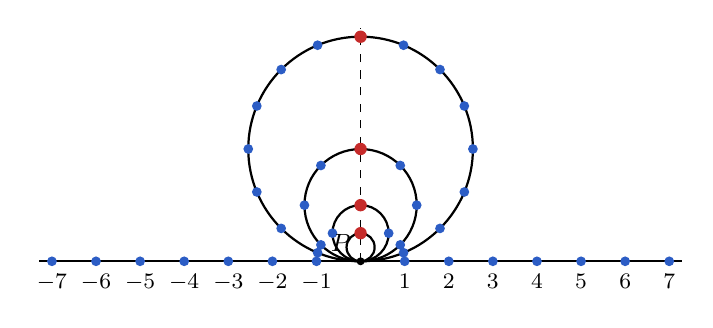
\begin{tikzpicture}[scale=0.8, every node/.style={font=\small}]
  \coordinate (P) at (0,0);
  % Circles and line share one scale: one unit of arc length (or of distance along the
  % line) is 0.7 here, so the circle of circumference 2^{k+1} has radius 0.7*2^k/pi.
  \draw[thick] (0,0.223) circle (0.223);
  \draw[thick] (0,0.446) circle (0.446);
  \draw[thick] (0,0.891) circle (0.891);
  \draw[thick] (0,1.783) circle (1.783);
  \draw[thin,dashed] (0,0)--(0,3.7);
  % Lamps on each circle: the circle of circumference 2^{k+1} carries one lamp at every
  % arc distance s=1,...,2^{k+1}-1; the antipode s=2^k is the spot the red lamp fills in.
  % The innermost circle, of circumference 2, has only that antipode lamp.
  \foreach \s [evaluate=\s as \ang using {180*\s/2-90}] in {1,3}
    \fill[lampB] (0,0.446) + (\ang:0.446) circle (2.2pt);
  \foreach \s [evaluate=\s as \ang using {180*\s/4-90}] in {1,2,3,5,6,7}
    \fill[lampB] (0,0.891) + (\ang:0.891) circle (2.2pt);
  \foreach \s [evaluate=\s as \ang using {180*\s/8-90}] in {1,2,3,4,5,6,7,9,10,11,12,13,14,15}
    \fill[lampB] (0,1.783) + (\ang:1.783) circle (2.2pt);
  \fill[lampA] (0,0.446) circle (2.8pt);
  \fill[lampA] (0,0.891) circle (2.8pt);
  \fill[lampA] (0,1.783) circle (2.8pt);
  \fill[lampA] (0,3.565) circle (2.8pt);
  \draw[thick] (-5.1,0)--(5.1,0);
  \foreach \x/\lab in {-4.9/-7,-4.2/-6,-3.5/-5,-2.8/-4,-2.1/-3,-1.4/-2,-0.7/-1,0.7/1,1.4/2,2.1/3,2.8/4,3.5/5,4.2/6,4.9/7} {
    \fill[lampB] (\x,0) circle (2.2pt);
    \node[below,font=\footnotesize] at (\x,-0.05) {$\lab$};
  }
  \fill (P) circle (1.8pt);
  \node[above left] at (P) {$P$};
\end{tikzpicture}
\caption{Red marks the lamp added each round.}
\label{fig:onepic}
\end{figure}

The difference from Sections 2.4--2.5 is a single one. There every round is a pure equivalent
replacement, the total brightness is conserved, and the limit reads off the odd terms; here
the brightness accumulates round by round, the price is one added lamp per round, and what is
bought is that the series \eqref{eq:basel} itself appears on the figure. Each term of
\eqref{eq:supplement-brightness} can be pointed at on the picture. Once the picture is drawn
the only computation left is a geometric series with ratio $\frac14$.

\section*{Acknowledgments}

The geometric construction is due to Johan W\"astlund; this note only takes one further step
on his figure. The exposition also benefited from the video version by 3Blue1Brown.

\begin{thebibliography}{9}

\bibitem{wastlund}
J.~W\"astlund, \emph{Summing inverse squares by euclidean geometry},
Chalmers University of Technology, Gothenburg, 8 December 2010.
Unpublished note.
\url{https://www.math.chalmers.se/~wastlund/Cosmic.pdf}

\bibitem{threeblueonebrown}
3Blue1Brown, \emph{Why is $\pi$ here? And why is it squared? A geometric answer to the
Basel problem}, YouTube, 3 March 2018.
\url{https://www.youtube.com/watch?v=d-o3eB9sfls}

\bibitem{kalman}
D.~Kalman, \emph{Six ways to sum a series}, College Mathematics Journal 24 (5), 402--421, 1993.

\bibitem{matsuoka}
Y.~Matsuoka, \emph{An elementary proof of the formula $\sum 1/k^{2}=\pi^{2}/6$},
American Mathematical Monthly 68 (5), 1961.

\bibitem{komornik}
V.~Komornik, \emph{A ``luminous'' solution to the Basel problem},
Mathematics Magazine 95 (4), 333--337, 2022.

\bibitem{wikipedia}
{Wikipedia contributors}, \emph{Basel problem}, section ``Geometric proof'', which reproduces
the construction of \cite{wastlund}.
\url{https://en.wikipedia.org/wiki/Basel_problem}, accessed 20 November 2026.

\end{thebibliography}


\end{document}
